\documentclass[xcolor=svgnames]{beamer}
\usetheme{Torino}

\usepackage{epsfig} %for figures
\usepackage{xcolor} %for color
\usepackage[utf8]{inputenc}
\usepackage{multicol}
\usepackage{hyperref}

% latex definitions:
\def\d{{\rm d}}
\def\half{{\textstyle{1\over2}}}



\title[SymPy\hspace{4em}\insertframenumber/
\inserttotalframenumber]{~\\ SymPy Tutorial \\~}


\author[A. Meurer, Matthew Rocklin, Jason Moore]
{Aaron Meurer, Ondřej Čertík, Amit Kumar, Jason Moore, \\ Sartaj Singh, Harsh Gupta}

\pgfdeclareimage[height=1.5cm]{mylogo}{sympy-250px}
\institute{\pgfuseimage{mylogo}}

\date{July 11, 2016}

\begin{document}

\begin{frame}
  \maketitle
\begin{center}
\normalsize All materials for today's tutorial are at \url{http://www.sympy.org/scipy-2016-tutorial/}
\end{center}
\end{frame}

\begin{frame}{Outline}
  \begin{block}{SymPy Introduction}
    \begin{itemize}
    \item Goal
    \item Features
    \item History
    \item Present
    \item Future
    \end{itemize}
  \end{block}

  \begin{block}{Tutorial}
    \begin{itemize}
    \item Intro to SymPy and Basic features
    \item Solving real life problems
    \end{itemize}
  \end{block}
\end{frame}

\begin{frame}{SymPy Goal}
  \begin{block}{Goal}
    Provide a symbolic manipulation library in Python.
  \end{block}
  \pause
  \begin{block}

    ``SymPy is an open source Python library for symbolic mathematics. It aims to
    become a full-featured computer algebra system (CAS) while keeping the code as
    simple as possible in order to be comprehensible and easily extensible. SymPy
    is written entirely in Python and does not require any external libraries.''

  \end{block}
\end{frame}

\begin{frame}{Why SymPy?}
  \begin{block}{}
    \begin{itemize}
      \item Standalone
      \item Full featured
      \item BSD licensed
      \item Embraces Python
      \item Usable as a library
    \end{itemize}
  \end{block}
\end{frame}

\begin{frame}{Features}
  \begin{multicols}{2}
    \tiny
    \begin{itemize}
    \item \textbf{Core Capabilities}
      \begin{itemize}
        \tiny
      \item Basic arithmetic: Support for operators such as +, -, *, /, ** (power)
      \item Simplification
      \item Expansion
      \item Functions: trigonometric, hyperbolic, exponential, roots, logarithms,
        absolute value, spherical harmonics, factorials and gamma functions, zeta
        functions, polynomials, special functions, \ldots
      \item Substitution
      \item Numbers: arbitrary precision integers, rationals, and floats
      \item Noncommutative symbols
      \item Pattern matching
      \end{itemize}
    \item \textbf{Polynomials}
      \begin{itemize}
        \tiny
      \item Basic arithmetic: division, gcd, \ldots
      \item Factorization
      \item Square-free decomposition
      \item Gröbner bases
      \item Partial fraction decomposition
      \item Resultants
      \end{itemize}
    \item \textbf{Calculus}
      \begin{itemize}
        \tiny
      \item Limits: $\lim_{x\to 0}{x\log(x)} = 0$
      \item Differentiation
      \item Integration: It uses extended Risch-Norman heuristic
      \item Taylor (Laurent) series
      \end{itemize}
    \item \textbf{Solving equations}
      \begin{itemize}
        \tiny
      \item Polynomial equations
      \item Algebraic equations
      \item Differential equations
      \item Difference equations
      \item Systems of equations
      \end{itemize}
    \item \textbf{Combinatorics}
      \begin{itemize}
        \tiny
      \item Permutations
      \item Combinations
      \item Partitions
      \item Subsets
      \item Permutation Groups: Polyhedral, Rubik, Symmetric, \ldots
      \item Prufer and Gray Codes
      \end{itemize}

    \end{itemize}
  \end{multicols}
\end{frame}

\begin{frame}{Features}
  \begin{multicols}{2}
    \begin{itemize}
      \tiny
    \item \textbf{Discrete math}
      \begin{itemize}
        \tiny
      \item Binomial coefficients
      \item Summations
      \item Products
      \item Number theory: generating prime numbers, primality testing, integer
        factorization, \ldots
      \item Logic expressions
      \end{itemize}

    \item \textbf{Matrices}
      \begin{itemize}
        \tiny
      \item Basic arithmetic
      \item Eigenvalues/eigenvectors
      \item Determinants
      \item Inversion
      \item Solving
      \item Abstract expressions
      \end{itemize}


    \item \textbf{Geometric Algebra}


    \item \textbf{Geometry}
      \begin{itemize}
        \tiny
      \item points, lines, rays, segments, ellipses, circles, polygons, \ldots
      \item Intersection
      \item Tangency
      \item Similarity
      \end{itemize}

    \item \textbf{Plotting}
      \begin{itemize}
        \tiny
      \item Coordinate modes
      \item Plotting Geometric Entities
      \item 2D and 3D
      \item Interactive interface
      \item Colors
      \end{itemize}

    \item \textbf{Physics}
      \begin{itemize}
        \tiny
      \item Units
      \item Mechanics
      \item Quantum
      \item Gaussian Optics
      \item Pauli Algebra
      \end{itemize}

    \item \textbf{Statistics}
      \begin{itemize}
        \tiny
      \item Normal distributions
      \item Uniform distributions
      \item Probability
      \end{itemize}

    \item \textbf{Printing}
      \begin{itemize}
        \tiny
      \item Pretty printing: ASCII/Unicode pretty printing, LaTeX
      \item Code generation: C, Fortran, Python
      \end{itemize}
    \end{itemize}
  \end{multicols}
\end{frame}

\begin{frame}{History}
  \begin{block}{History}
    \begin{itemize}
    \item Ondřej Čertík started the project in 2006.
    \item Development took off in 2007 when SymPy first participated in Google
      Summer of Code. We have participated in every Google Summer of Code since.
    \item In 2011, Aaron Meurer (who also joined from Google Summer of Code) took
      over as lead developer.
    \end{itemize}
  \end{block}
\end{frame}

\begin{frame}{Present}
  \begin{block}{Current Status}
    \begin{itemize}
    \item Over 450 contributors.
    \item Current code base has over 400,000 lines of code and documentation.
    \item We have crossed the point of ``sympy a toy'' to ``sympy a tool''
    \end{itemize}
  \end{block}
\end{frame}

\begin{frame}{Future}
  \begin{block}{GSoC (1/2)}
    These are our current GSoC projects. Expect to see these features by the end
    of the summer.
    \begin{itemize}
    \item \normalsize Group Theory, \small Gaurav Dhingra
    \item \normalsize Extending solveset, \small Kshitij Saraogi
    \item \normalsize Completing Solveset, \small Shekhar Prasad Rajak
    \item \normalsize Implementation of Holonomic Functions, \small Shubham Tibra
    \item \normalsize Implementation of Singularity Functions to solve Beam Bending problems, \small Sampad Kumar Saha

    \end{itemize}
  \end{block}
\end{frame}

\begin{frame}{Future}
  \begin{block}{GSoC (2/2)}
    These are our current GSoC projects. Expect to see these features by the end
    of the summer.
    \begin{itemize}
    \item \normalsize Adding to SymEngine's Polynomial functionality and interfacing it with FLINT \& Piranha \small Srajan Garg
    \item \normalsize Implementing Finite Fields and Set module in SymEngine \small Nishant Nikhil
    \end{itemize}
  \end{block}
\end{frame}

\begin{frame}{Future}
\begin{block}{Other Plans}
\begin{itemize}
\item New assumptions
\item Make things faster
\item SymEngine (\url{https://github.com/symengine})
\item Implement more algorithms, so we can compute more things (and also make
  them faster)
\item Replacing \texttt{solve} with \texttt{solveset}
\item Encourage people to use SymPy for many applications
\item \url{https://github.com/sympy/sympy/wiki/gsoc-2016-ideas} for full list of
  things we want done
\end{itemize}
\end{block}
\end{frame}


%% I was too lazy to redo these for now

%% \begin{frame}{Git Commits Plots}
%%   \begin{block}{Last Year}
%%     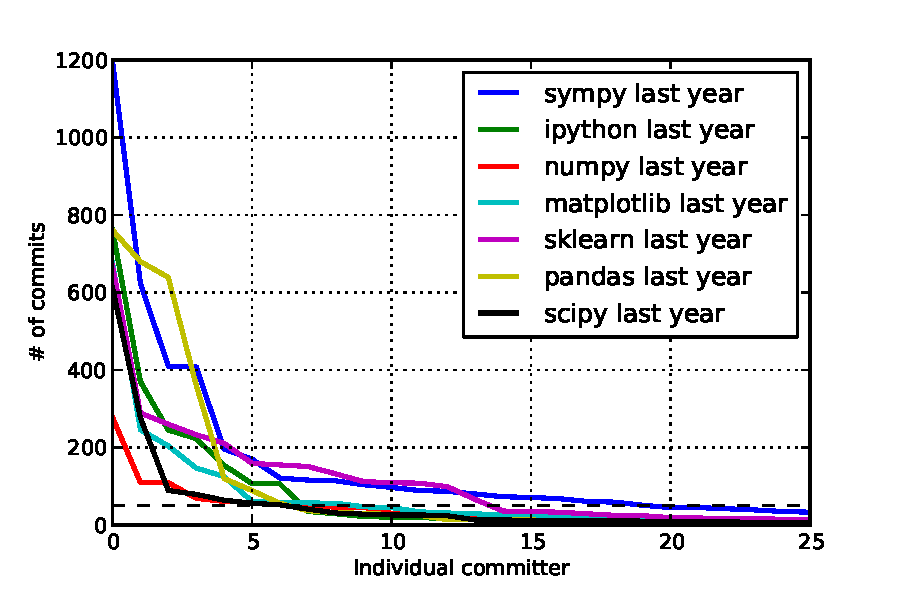
\includegraphics[width=4in]{commits1.pdf}
%%   \end{block}
%% \end{frame}
%%
%% \begin{frame}{Git Commit Plots}
%%   \begin{block}{Last Year}
%%     \begin{itemize}
%%     \item The dotted line is 50 commits.
%%     \item Rough measurement of each project's ``bus factor''
%%     \end{itemize}
%%   \end{block}
%% \end{frame}
%%
%% \begin{frame}{Git Commits Plots}
%%   \begin{block}{All Time}
%%     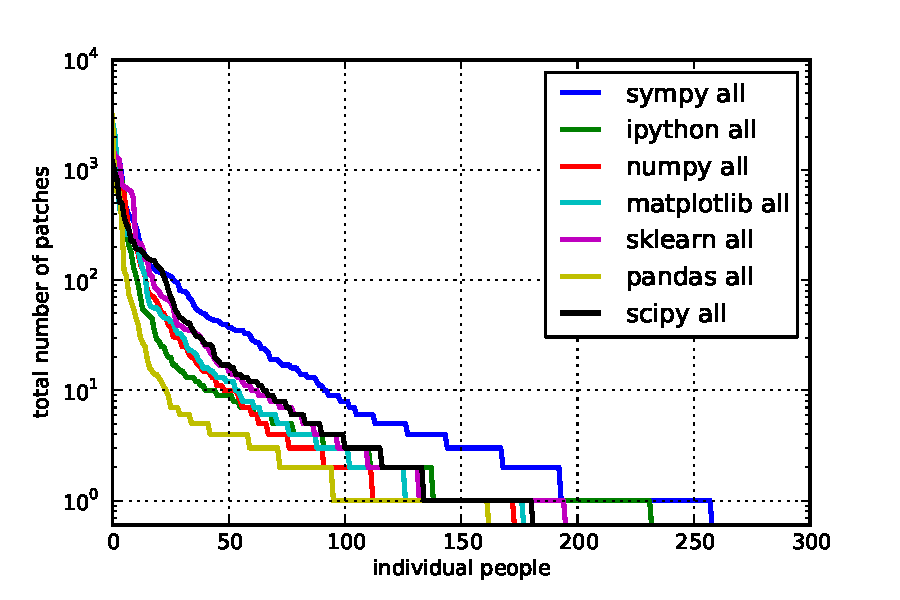
\includegraphics[width=4in]{commits-all.pdf}
%%   \end{block}
%% \end{frame}
%%
%% \begin{frame}{Git Commit Plots}
%%   \begin{block}{All Time}
%%     \begin{itemize}
%%     \item SymPy has more total contributors\footnote{some of the other projects are actually exaggerated,
%%         because they don't use \texttt{.mailmap}}
%%     \item SymPy has a very welcome and friendly community, which is open, and
%%       actively encourages contributions.
%%     \item The SymPy code base is very approachable to new contributors.
%%     \item To be fair, Google Code-In accounts for a lot of this\ldots
%%     \end{itemize}
%%   \end{block}
%% \end{frame}


\begin{frame}{Projects Using SymPy}
\begin{itemize}
\item
  \href{http://www.sagemath.org/}{\textbf{Sage}}: A CAS, visioned to be
  a viable free open source alternative to Magma, Maple, Mathematica and
  MATLAB\@. Sage includes many open source mathematical libraries, including
  SymPy.
\item
  \href{https://cloud.sagemath.com}{\textbf{SageMathCloud}}:
  SageMathCloud is a web-based cloud computing and course management
  platform for computational mathematics.
\item
  \href{http://mathpix.com/}{\textbf{Mathpix}}: An iOS App, that detects
  handwritten math as input, and uses SymPy Gamma to evaluate the math input
  and generate the relevant steps to solve the problem.
\item
  \href{http://www.pydy.org/}{\textbf{PyDy}}: Multibody Dynamics with
  Python.
\item
  \href{http://openrave.org/docs/0.8.2/openravepy/ikfast/}{\textbf{IKFast}}:
  IKFast is a robot kinematics compiler provided by
  \href{http://openrave.org/}{OpenRAVE}. It analytically solves robot inverse
  kinematics equations and generates optimized C++ files. It uses SymPy for
  its internal symbolic mathematics.
\end{itemize}
  \end{frame}

\begin{frame}{Projects Using SymPy}
\begin{itemize}
\item
  \href{http://octave.sourceforge.net/symbolic/}{\textbf{Octave Symbolic}}:
  The Octave-Forge Symbolic package adds symbolic calculation features
  to GNU Octave. These include common CAS tools such
  as algebraic operations, calculus, equation solving, Fourier and
  Laplace transforms, variable precision arithmetic, and other features.
\item
  \href{https://github.com/brombo/galgebra}{\textbf{galgebra}}:
  Geometric algebra (previously \texttt{sympy.galgebra}).
\item
  \href{https://github.com/jverzani/SymPy.jl}{\textbf{SymPy.jl}}:
  Provides a Julia interface to SymPy using PyCall.
\item
  \href{https://mathics.github.io/}{\textbf{Mathics}}: Mathics is a
  free, general-purpose online CAS featuring Mathematica compatible
  syntax and functions. It is backed by highly extensible Python code,
  relying on SymPy for most mathematical tasks.
\item
  \href{http://sfepy.org/}{\textbf{SfePy}}: Simple finite elements in
  Python.
\end{itemize}
\end{frame}

\begin{frame}{Projects Using SymPy}
\begin{itemize}
\item
  \href{http://quameon.sourceforge.net/}{\textbf{Quameon}}: Quantum
  Monte Carlo in Python.
\item
  \href{http://lcapy.elec.canterbury.ac.nz/}{\textbf{Lcapy}}:
  Experimental Python package for teaching linear circuit analysis.
\item
  \href{http://digitalcommons.calpoly.edu/cgi/viewcontent.cgi?article=1072\&context=physsp/}{\textbf{Quantum
  Programming in Python}}: Quantum 1D Simple Harmonic Oscillator and
  Quantum Mapping Gate.
\item
  \href{http://mech.fsv.cvut.cz/~stransky/software/latexexpr/doc/}{\textbf{LaTeX
  Expression project}}: Easy \LaTeX{} typesetting of algebraic expressions
  in symbolic form with automatic substitution and result computation.
\item
  \href{https://www.researchgate.net/publication/260585491_Symbolic_Statistics_with_SymPy/}{\textbf{Symbolic
  statistical modeling}}: Adding statistical operations to complex
  physical models.
\end{itemize}
\end{frame}

\begin{frame}{Authors}
\begin{multicols}{5}
\tiny
Chris Smith\\
Aaron Meurer\\
Mateusz Paprocki\\
Ondřej Čertík\\
Sergey B Kirpichev\\
Matthew Rocklin\\
Julien Rioux\\
Raoul Bourquin\\
Ronan Lamy\\
Kirill Smelkov\\
Øyvind Jensen\\
Tom Bachmann\\
Sudhanshu Mishra\\
Mario Pernici\\
AMiT Kumar\\
Sergiu Ivanov\\
Jason Moore\\
Sachin Joglekar\\
Colin B. Macdonald\\
Gaurav Dhingra\\
Sartaj Singh\\
Saptarshi Mandal\\
Sean Vig\\
Thilina Rathnayake\\
Jim Crist\\
Stefan Krastanov\\
Francesco Bonazzi\\
David Li\\
Brian E. Granger\\
Rick Muller\\
Kalevi Suominen\\
Shubham Tibra\\
Vinzent Steinberg\\
Timothy Reluga\\
Gilbert Gede\\
Vladimir Perić\\
Raymond Wong\\
Thomas Hisch\\
Harsh Gupta\\
Shivam Vats\\
Fredrik Johansson\\
Fabian Pedregosa\\
Bharath M R\\
Addison Cugini\\
Kundan Kumar\\
Joachim Durchholz\\
Peter Brady\\
Guru Devanla\\
Manoj Kumar\\
Alexey U. Gudchenko\\
hm\\
Björn Dahlgren\\
Priit Laes\\
Prasoon Shukla\\
Matt Habel\\
Alan Bromborsky\\
Robert Johansson\\
Juha Remes\\
Tomo Lazovich\\
Matt Curry\\
Mary Clark\\
Pablo Puente\\
Harold Erbin\\
Sampad Kumar Saha\\
Jason Gedge\\
Ramana Venkata\\
Christopher Dembia\\
Aleksandar Makelov\\
Katja Sophie Hotz\\
Brian Jorgensen\\
Chai Wah Wu\\
Kendhia\\
Akshay\\
Andy R. Terrel\\
Grzegorz Świrski\\
Pearu Peterson\\
Sebastian Krämer\\
Alkiviadis G. Akritas\\
Anurag Sharma\\
Joan Creus\\
Siddhanathan Shanmugam\\
Toon Verstraelen\\
Cristóvão Sousa\\
Christian Muise\\
Jorn Baayen\\
Jeremias Yehdegho\\
Sahil Shekhawat\\
Thomas Baruchel\\
Alexander Hirzel\\
Kevin Hunter\\
Matthew Hoff\\
Riccardo Gori\\
Tanu Hari Dixit\\
Shipra Banga\\
Meghana Madhyastha\\
Steve Anton\\
Oliver Lee\\
Sanket Agarwal\\
Dustin Gadal\\
Jason Siefken\\
Mark Dewing\\
rathmann\\
Jatin Yadav\\
Robert Schwarz\\
David Ju\\
Keval Shah\\
Luke Peterson\\
Angadh Nanjangud\\
Arafat Dad Khan\\
Stephen Loo\\
\end{multicols}
\end{frame}
\begin{frame}{Authors (continued)}
\begin{multicols}{5}
\tiny
Comer Duncan\\
Kshitij Saraogi\\
Renato Coutinho\\
Yuriy Demidov\\
Bilal Akhtar\\
Stepan Roucka\\
Alex Lindsay\\
Chetna Gupta\\
Dzhelil Rufat\\
Miha Marolt\\
Peleg Michaeli\\
Amit Saha\\
Soumya Dipta Biswas\\
Ralf Stephan\\
Randy Heydon\\
Saurabh Jha\\
arihant parsoya\\
Aravind Reddy\\
Nathan Alison\\
Niklas Thörne\\
YiDing Jiang\\
James Brandon Milam\\
Kyle McDaniel\\
Peter Schmidt\\
jerryma1121\\
Ashutosh Saboo\\
Brian Stephanik\\
Robert Kern\\
Sachin Irukula\\
Sam Sleight\\
Angus Griffith\\
Avichal Dayal\\
Pablo Zubieta\\
Patrick Lacasse\\
Swapnil Agarwal\\
Anthony Scopatz\\
Gary Kerr\\
Anish Shah\\
Mike Boyle\\
Natalia Nawara\\
Nicolas Pourcelot\\
Rishabh Daal\\
Sherjil Ozair\\
Aaditya Nair\\
Ankit Agrawal\\
Harshil Goel\\
Huijun Mai\\
Jim Zhang\\
Ljubiša Moćić\\
Mark Shoulson\\
Prafullkumar P. Tale\\
Marek Šuppa\\
Akash Trehan\\
Akshay Siramdas\\
Chaitanya Sai Alaparthi\\
Freddie Witherden\\
Richard Otis\\
Roberto Nobrega\\
kshitij10496\\
David Joyner\\
Felix Kaiser\\
Lennart Fricke\\
Mihir Wadwekar\\
Min Ragan-Kelley\\
Shekhar Prasad Rajak\\
Curious72\\
Friedrich Hagedorn\\
Jennifer White\\
Saroj Adhikari\\
Sean Ge\\
Zamrath Nizam\\
Aditya Shah\\
Alexey Subach\\
CJ Carey\\
Eric Nelson\\
Jaroslaw Tworek\\
Longqi Wang\\
Michael Boyle\\
Moo VI\\
Nitin Chaudhary\\
Yuri Karadzhov\\
Abhishek Verma\\
Alex Argunov\\
Christian Bühler\\
David T\\
Devyani Kota\\
Isuru Fernando\\
Matthew Brett\\
Rajat Aggarwal\\
Rishabh Dixit\\
Ryan Krauss\\
Ananya H\\
Andreas Kloeckner\\
Dammina Sahabandu\\
Dana Jacobsen\\
Demian Wassermann\\
Duane Nykamp\\
Eva Charlotte Mayer\\
Gao, Xiang\\
Kumar Krishna Agrawal\\
Raphael Michel\\
Sam Magura\\
Sumith\\
Tim Swast\\
carstimon\\
Adam Bloomston\\
Bhautik Mavani\\
Chancellor Arkantos\\
Chris Wu\\
Christophe Saint-Jean\\
\end{multicols}
\end{frame}
\begin{frame}{Authors (continued)}
\begin{multicols}{5}
\tiny
David P. Sanders\\
Davy Mao\\
Jiaxing Liang\\
Khagesh Patel\\
Manish Gill\\
Matthew Thomas\\
Nichita Utiu\\
Piotr Korgul\\
Roland Puntaier\\
Ruslan Pisarev\\
Tarun Gaba\\
Tobias Lenz\\
Tomasz Buchert\\
richierichrawr\\
Abderrahim Kitouni\\
Akshay Nagar\\
Alexander Bentkamp\\
Alexandr Popov\\
Aman Deep\\
Archit Verma\\
Ben Lucato\\
Boris Atamanovskiy\\
Chak-Pong Chung\\
Chris Conley\\
ChristinaZografou\\
David Roberts\\
Florian Mickler\\
Haruki Moriguchi\\
Imran Ahmed Manzoor\\
Jai Luthra\\
Jochen Voss\\
Juan Felipe Osorio\\
Leonid Blouvshtein\\
Lokesh Sharma\\
Michał Radwański\\
Nguyen Truong Duy\\
Nimish Telang\\
Pramod Ch\\
Rom le Clair\\
Sanya Khurana\\
Sebastian Kreft\\
Shashank Agarwal\\
Stas Kelvich\\
Stefan van der Walt\\
Stefano Maggiolo\\
Stefen Yin\\
Tiffany Zhu\\
Tom Gijselinck\\
Tristan Hume\\
Varun Joshi\\
Zeel Shah\\
Óscar Nájera\\
Abhinav Agarwal\\
Akshay Srinivasan\\
Akshit Agarwal\\
Amit Jamadagni\\
Andrew Straw\\
Barry Wardell\\
Benjamin McDonald\\
Bill Flynn\\
Buck Shlegeris\\
Case Van Horsen\\
Craig A. Stoudt\\
Darshan Chaudhary\\
Edward Schembor\\
Emma Hogan\\
Eric Miller\\
Geoffry Song\\
George Waksman\\
Hamish Dickson\\
Heiner Kirchhoffer\\
Jens H. Nielsen\\
Julio Idichekop Filho\\
Kaushik Varanasi\\
Kevin Ventullo\\
Luca Weihs\\
Luis Garcia\\
Manoj Babu K.\\
Martin Povišer\\
Mathew Chong\\
Matthew Parnell\\
Mridul Seth\\
Nikolay Lazarov\\
Oscar Benjamin\\
Pan Peng\\
Phillip Berndt\\
Raffaele De Feo\\
Renato Orsino\\
Sarwar Chahal\\
Shravas K Rao\\
Sunny Aggarwal\\
Ted Dokos\\
Ted Horst\\
Tschijnmo TSCHAU\\
Tuomas Airaksinen\\
Vasiliy Dommes\\
Venkatesh Halli\\
operte\\
Abhishek Garg\\
Alec Kalinin\\
Anton Akhmerov\\
Arpit Goyal\\
Ashwini Oruganti\\
Asish Panda\\
Ben Goodrich\\
Boris Timokhin\\
Bradley Froehle\\
Cody Herbst\\
Colleen Lee\\
David Marek\\
\end{multicols}
\end{frame}
\begin{frame}{Authors (continued)}
\begin{multicols}{5}
\tiny
Dimitra Konomi\\
Dmitry Batkovich\\
Fernando Perez\\
FiachAntaw\\
Goutham Lakshminarayan\\
Henrik Johansson\\
Henry Gebhardt\\
Jack McCaffery\\
James Aspnes\\
James Fiedler\\
Jayesh Lahori\\
Jezreel Ng\\
John V. Siratt\\
Juan Luis Cano Rodríguez\\
Jurjen N.E. Bos\\
Justin Blythe\\
Konstantin Togoi\\
Krit Karan\\
Kunal Arora\\
Laura Domine\\
Lukas Zorich\\
Luv Agarwal\\
Maciej Baranski\\
Matthew Davis\\
Michael Mayorov\\
Michael Mueller\\
Michael S. Hansen\\
Nikhil Sarda\\
Oleksandr Gituliar\\
Param Singh\\
Patrick Poitras\\
Pavel Fedotov\\
Phil Ruffwind\\
Pradyumna\\
QuaBoo\\
Rajath Shashidhara\\
Rehas Sachdeva\\
Roman Inflianskas\\
Sai Nikhil\\
Shivam Tyagi\\
Shukla\\
Sushant Hiray\\
Thomas Dixon\\
Thomas Wiecki\\
Tomáš Bambas\\
Tuan Manh Lai\\
Vladimir Poluhsin\\
Yu Kobayashi\\
Yury G. Kudryashov\\
bluebrook\\
tsmars15\\
Abhinav Chanda\\
Akshat Jain\\
Alexander Eberspächer\\
Alexandr Gudulin\\
Ali Raza Syed\\
Alistair Lynn\\
Ambar Mehrotra\\
Anatolii Koval\\
Andre de Fortier Smit\\
Andrej Tokarčík\\
Andrew Docherty\\
Aqnouch Mohammed\\
Bastian Weber\\
Benjamin Fishbein\\
Benjamin Gudehus\\
Bernhard R. Link\\
Carsten Knoll\\
Chris Swierczewski\\
Christian Schubert\\
Clemens Novak\\
David Lawrence\\
Dhruvesh Vijay Parikh\\
Eh Tan\\
Elrond der Elbenfuerst\\
Erik Welch\\
Faisal Anees\\
Fawaz Alazemi\\
G. D. McBain\\
Gert-Ludwig Ingold\\
GitRay\\
GolimarOurHero\\
Govind Sahai\\
Gregory Ashton\\
Gregory Ksionda\\
Guillaume Gay\\
Guillaume Jacquenot\\
Guo Xingjian\\
Haimo Zhang\\
Hubert Tsang\\
Jack Kemp\\
Jacob Garber\\
James Abbatiello\\
James Goppert\\
James Pearson\\
Jason Ly\\
Jens Jørgen Mortensen\\
Jeremy\\
Jerry Li\\
Johann Cohen-Tanugi\\
John Connor\\
Jonathan Miller\\
Jorge E. Cardona\\
Joseph Dougherty\\
Josh Burkart\\
Kaifeng Zhu\\
Kazuo Thow\\
Kevin Goodsell\\
Kibeom Kim\\
Konrad Meyer\\
\end{multicols}
\end{frame}
\begin{frame}{Authors (continued)}
\begin{multicols}{5}
\tiny
Langston Barrett\\
Lars Buitinck\\
Lucas Jones\\
Madeleine Ball\\
Marcin Kostrzewa\\
Marcus Näslund\\
Markus Müller\\
Matt Rajca\\
Matthew Tadd\\
Matthias Toews\\
Max Hutchinson\\
Michael Gallaspy\\
Michael Zingale\\
Mihai A. Ionescu\\
Nathan Musoke\\
Nathan Woods\\
Nicholas J.S. Kinar\\
Nicolás Guarín-Zapata\\
Nishant Nikhil\\
Nishith Shah\\
Normal Human\\
Or Dvory\\
Pastafarianist\\
Paul Scott\\
Paul Strickland\\
Pauli Virtanen\\
Philippe Bouafia\\
Pierre Haessig\\
Prabhjot Singh\\
Prashant Tyagi\\
Prateek Papriwal\\
Prempal Singh\\
Puneeth Chaganti\\
Raj\\
Ralph Bean\\
Ray Cathcart\\
Rich LaSota\\
Rizgar Mella\\
Robert\\
Robert Cimrman\\
Roberto Colistete, Jr.\\
Sam Tygier\\
Sambuddha Basu\\
Sandeep Veethu\\
Sebastian Koslowski\\
Sebastian Krause\\
Seshagiri Prabhu\\
Shai 'Deshe' Wyborski\\
Shashank Kumar\\
Shruti Mangipudi\\
Siddhant Jain\\
Sourav Singh\\
Srajan Garg\\
Srinivas Vasudevan\\
Stepan Simsa\\
Subham Tibra\\
Sumith1896\\
Takafumi Arakaki\\
Tarang Patel\\
Thomas Hickman\\
Thomas Sidoti\\
Tim Lahey\\
Timothy Cyrus\\
Tyler Pirtle\\
Vasily Povalyaev\\
Venkata Ramana\\
Victor Brebenar\\
Vinay\\
Vinay Kumar\\
Vinit Ravishankar\\
Vlad Seghete\\
Vladimir Lagunov\\
ck Lux\\
dustyrockpyle\\
immerrr\\
mao8\\
marshall2389\\
sevaader\\
siddharthist\\
vishal\\
zsc347\\
Łukasz Pankowski\\
\end{multicols}
\end{frame}


\begin{frame}{Here at SciPy}
  \begin{block}{Talks}
    \begin{itemize}
    \item \normalsize Jason Moore, \textit{Simulating Robot, Vehicle, Spacecraft, and Animal Motion with Python (Advanced)}
      (Tutorial). \\ \footnotesize Monday 1:30 PM - 5:30 PM - Room 103
    \item \normalsize Aaron Meurer, Anthony Scopatz \textit{SymPy Code Generation}. \\ \footnotesize Thursday 11:30
      PM - 12:00 PM - Room 204
    \item \normalsize Ondřej Čertík, Isuru Fernando, Thilina Rathnayake, Abhinav Agarwal \textit{SymEngine: A Fast Symbolic Manipulation Library}. \\ \footnotesize Friday 3:30
      - 4:00 - Room 204
    \end{itemize}
  \end{block}
\end{frame}

%\begin{frame}{Here at SciPy}
%  \begin{block}{Bof}
%    \begin{itemize}
%      \item SymPy BoF - Wednesday 5:30 PM - 6:30 PM - Rm 203
%    \end{itemize}
%  \end{block}
%  \begin{block}{Sprints}
%    Come sprint with us!
%    \begin{itemize}
%    \item Releasing SymPy 1.1
%    \item Assumptions
%    \item Whatever interests you
%    \item Lot's of tasks that are easy for new contributors
%    \item Friday and Saturday
%    \end{itemize}
%  \end{block}
%\end{frame}

\begin{frame}
\Huge Let's begin!
\end{frame}
\end{document}
